% Préambule commun des schémas TikZ (compilés séparément par construire_figures.py)
\documentclass[tikz,border=3pt]{standalone}
\usepackage[T1]{fontenc}
\usepackage[utf8]{inputenc}
\usepackage{lmodern}
\usepackage{amsmath,amssymb}
\usepackage{bm}
\usepackage[american,siunitx,straightvoltages]{circuitikz}
\usetikzlibrary{arrows.meta,positioning,calc,decorations.pathmorphing,
  decorations.markings,decorations.pathreplacing,patterns,shapes.geometric,
  shapes.misc,shapes.multipart,fit,backgrounds,3d,intersections,matrix}

\ctikzset{bipoles/length=1.1cm, amplifiers/scale=0.85, tripoles/op amp/width=1.4}

\tikzset{
  >={Latex[length=2mm,width=1.4mm]},
  every picture/.style={line width=0.6pt, font=\small},
  % schémas-blocs
  bloc/.style={draw, minimum width=1.5cm, minimum height=0.9cm, align=center,
               inner sep=3pt, fill=white},
  somme/.style={draw, circle, minimum size=4.5mm, inner sep=0pt, fill=white,
                path picture={\draw (path picture bounding box.north west)
                  -- (path picture bounding box.south east)
                  (path picture bounding box.north east)
                  -- (path picture bounding box.south west);}},
  gain/.style={draw, isosceles triangle, isosceles triangle apex angle=60,
               minimum size=8mm, inner sep=1pt, fill=white},
  bruit/.style={draw, circle, minimum size=4.5mm, inner sep=0pt, fill=white,
                path picture={\node at (path picture bounding box.center)
                  {\scriptsize$\ast$};}},
  cadre/.style={draw, dashed, rounded corners=1pt},
  cadrept/.style={draw, dash dot, rounded corners=1pt},
  fleche/.style={->},
  % mécanique
  bati/.style={pattern=north east lines, draw=none},
  ressort/.style={decorate, decoration={coil, aspect=0.4, segment length=2.2mm,
                  amplitude=2mm, pre length=2mm, post length=2mm}},
  zigzag/.style={decorate, decoration={zigzag, segment length=2mm,
                  amplitude=1.6mm, pre length=2mm, post length=2mm}},
  pivot/.style={draw, circle, fill=white, minimum size=2.2mm, inner sep=0pt},
  masse/.style={draw, fill=gray!25, minimum width=1.4cm, minimum height=0.8cm},
  cote/.style={<->, line width=0.4pt},
  axe/.style={->, line width=0.6pt},
  trait mixte/.style={dash dot, line width=0.4pt},
}

% Encastrement / bâti hachuré : \bati{(x1,y1)}{(x2,y2)} trace une ligne et ses hachures dessous
\newcommand{\bati}[3][0.18]{%
  \fill[pattern=north east lines] #2 rectangle ($#3+(0,-#1)$);
  \draw[line width=0.8pt] #2 -- #3;}

% Transducteur (deux cercles entrelacés) : \pic (t) at (x,y) {transducteur};  -> (t-o) entrée, (t-e) sortie
\tikzset{
  transducteur/.pic={\draw (-0.13,0) circle (0.24); \draw (0.13,0) circle (0.24);
    \coordinate (-o) at (-0.37,0); \coordinate (-e) at (0.37,0);
    \coordinate (-n) at (0,0.24); \coordinate (-s) at (0,-0.24);},
  bobine/.style={decorate, decoration={coil, aspect=0.7, segment length=1.4mm,
                 amplitude=1.6mm, pre length=1mm, post length=1mm}},
  sourcebruit/.style={draw, circle, minimum size=5mm, inner sep=0pt, fill=white,
                 label={[inner sep=0pt]center:$\ast$}},
  sourcecourant/.style={draw, circle, minimum size=5mm, inner sep=0pt, fill=white,
                 label={[inner sep=0pt]center:$\circledast$}},
}

% Composants compacts (pour les petits boîtiers des schémas-blocs)
\newcommand{\resistance}[2]{% de #1 à #2 (quelconque)
  \draw #1 -- ($#1!0.22!#2$) ($#1!0.78!#2$) -- #2;
  \draw[decorate, decoration={zigzag, segment length=1.5mm, amplitude=1.1mm}]
    ($#1!0.22!#2$) -- ($#1!0.78!#2$);}
\newcommand{\condensateur}[2]{% horizontal de #1 à #2
  \draw #1 -- ($($#1!0.5!#2$)+(-0.05,0)$) ($($#1!0.5!#2$)+(0.05,0)$) -- #2;
  \draw[line width=1pt] ($($#1!0.5!#2$)+(-0.05,0.14)$) -- ($($#1!0.5!#2$)+(-0.05,-0.14)$)
                        ($($#1!0.5!#2$)+(0.05,0.14)$) -- ($($#1!0.5!#2$)+(0.05,-0.14)$);}
% R // C horizontal : \RparC{(x,y)}{longueur}{écart}  (centre, longueur totale, écart vertical)
\newcommand{\RparC}[3]{%
  \coordinate (rcA) at ($#1+(-#2/2,0)$); \coordinate (rcB) at ($#1+(#2/2,0)$);
  \draw (rcA) -- ++(0.15,0) coordinate (rcA1) (rcB) -- ++(-0.15,0) coordinate (rcB1);
  \draw (rcA1) -- ++(0,#3/2) (rcA1) -- ++(0,-#3/2) (rcB1) -- ++(0,#3/2) (rcB1) -- ++(0,-#3/2);
  \resistance{($(rcA1)+(0,#3/2)$)}{($(rcB1)+(0,#3/2)$)}
  \condensateur{($(rcA1)+(0,-#3/2)$)}{($(rcB1)+(0,-#3/2)$)}}

\begin{document}
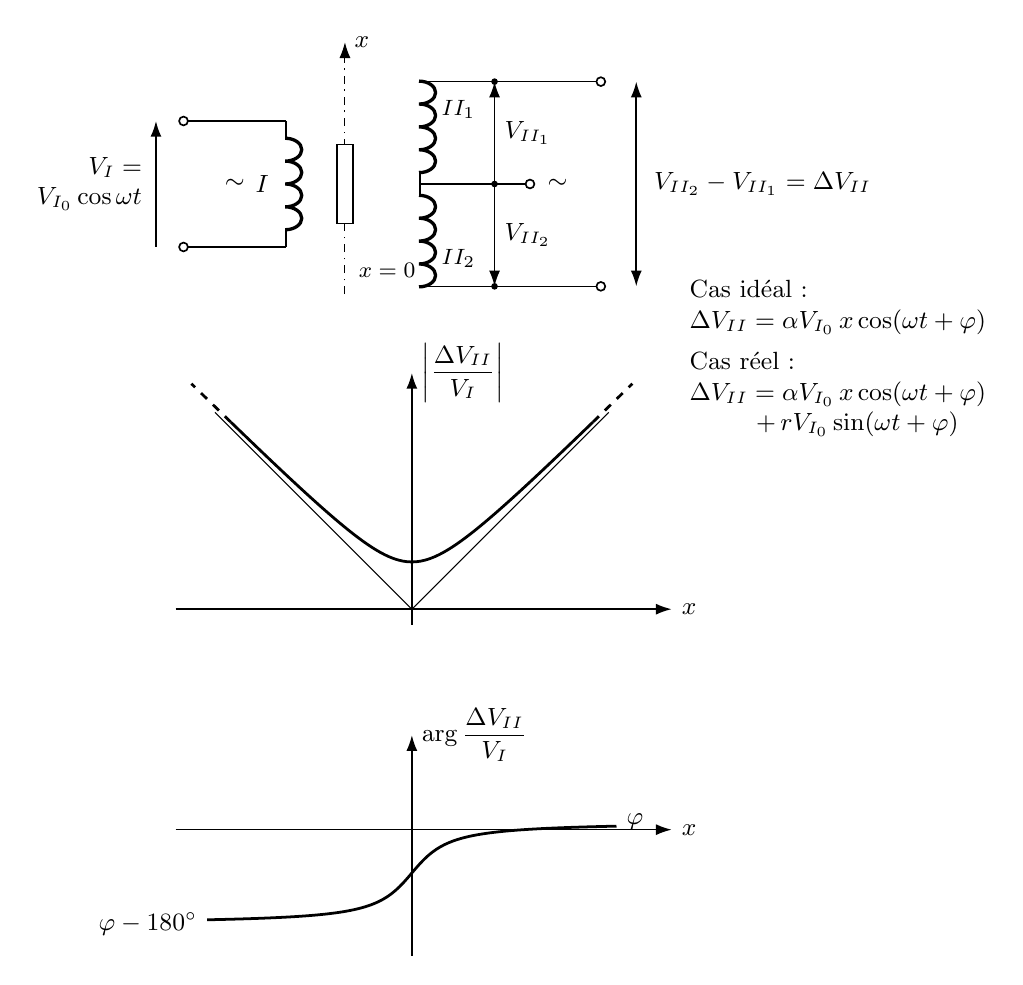
\begin{tikzpicture}[font=\small]
  % ---------- transformateur ----------
  \draw (0,1.6) node[ocirc] {} -- (1.3,1.6);
  \draw (0,0) node[ocirc] {} -- (1.3,0);
  \draw (1.3,1.6) to[L] (1.3,0);
  \node at (0.65,0.8) {$\sim$};
  \draw[->] (-0.35,0) -- (-0.35,1.6);
  \node[left, align=right] at (-0.4,0.8) {$V_I =$\\$V_{I_0}\cos\omega t$};
  \node at (1.0,0.8) {$I$};
  \draw[trait mixte, ->] (2.05,-0.6) -- (2.05,2.6) node[right] {$x$};
  \draw[fill=white] (1.95,0.3) rectangle (2.15,1.3);
  \node[right, font=\footnotesize] at (2.1,-0.3) {$x=0$};
  \draw (3.0,2.1) to[L] (3.0,0.95);
  \draw (3.0,0.65) to[L] (3.0,-0.5);
  \node[right, font=\footnotesize] at (3.15,1.75) {$II_1$}; \node[right, font=\footnotesize] at (3.15,-0.15) {$II_2$};
  \draw (3.0,2.1) -- (5.3,2.1) node[ocirc] {};
  \draw (3.0,0.95) -- (3.0,0.65);
  \draw (3.0,0.8) -- (4.4,0.8) node[ocirc] {};
  \draw (3.0,-0.5) -- (5.3,-0.5) node[ocirc] {};
  \fill (3.95,2.1) circle (1.2pt) (3.95,0.8) circle (1.2pt) (3.95,-0.5) circle (1.2pt);
  \draw[->] (3.95,0.8) -- (3.95,2.1) node[midway, right] {$V_{II_1}$};
  \draw[->] (3.95,0.8) -- (3.95,-0.5) node[midway, right] {$V_{II_2}$};
  \node at (4.75,0.8) {$\sim$};
  \draw[<->] (5.75,2.1) -- (5.75,-0.5);
  \node[right] at (5.85,0.8) {$V_{II_2} - V_{II_1} = \Delta V_{II}$};
  \node[align=left, anchor=north west] at (6.3,-0.3)
    {Cas idéal :\\$\Delta V_{II} = \alpha V_{I_0}\,x\cos(\omega t+\varphi)$\\[4pt]
     Cas réel :\\$\Delta V_{II} = \alpha V_{I_0}\,x\cos(\omega t+\varphi)$\\
     \hspace{2.6em}$+\, r V_{I_0}\sin(\omega t+\varphi)$};
  % ---------- module ----------
  \begin{scope}[shift={(2.9,-4.6)}]
    \draw[->] (-3.0,0) -- (3.3,0) node[right] {$x$};
    \draw[->] (0,-0.2) -- (0,3.0) node[right] {$\left|\dfrac{\Delta V_{II}}{V_I}\right|$};
    \draw[thin] (-2.5,2.5) -- (0,0) -- (2.5,2.5);
    \draw[line width=1pt, domain=-2.3:2.3, samples=81] plot (\x, {sqrt(\x*\x + 0.36)});
    \draw[line width=1pt, dashed] (-2.3,{sqrt(2.3*2.3+0.36)}) -- (-2.8,{sqrt(2.8*2.8+0.36)})
                                  (2.3,{sqrt(2.3*2.3+0.36)}) -- (2.8,{sqrt(2.8*2.8+0.36)});
  \end{scope}
  % ---------- phase ----------
  \begin{scope}[shift={(2.9,-7.4)}]
    \draw[->] (-3.0,0) -- (3.3,0) node[right] {$x$};
    \draw[->] (0,-1.6) -- (0,1.2) node[right] {$\arg\dfrac{\Delta V_{II}}{V_I}$};
    \draw[line width=1pt, domain=-2.6:2.6, samples=101]
      plot (\x, {-0.55 + 1.3/pi*atan2(\x, 0.6)/90*pi/2 *0 + (atan(\x/0.35)/180)*1.3});
    \node[right] at (2.6,0.1) {$\varphi$};
    \node[left] at (-2.6,-1.2) {$\varphi - 180^\circ$};
  \end{scope}
\end{tikzpicture}
\end{document}
